\documentclass{article}
\usepackage{graphicx} % Required for inserting images
\usepackage[utf8]{inputenc}
\usepackage[a4paper, margin = 1in]{geometry}
\usepackage{hyperref}
\usepackage{setspace}
\usepackage[inkscapelatex=false]{svg}
\usepackage{fontawesome}
\usepackage{booktabs}

\usepackage{array}
\usepackage{tabularx}


% Fix paragraph formatting
\setlength{\parindent}{0pt}
\setlength{\parskip}{0.5\baselineskip}


% TODO: Replace this title with actual peoject title. 
\title{PQ7: Tell Your Story}
\author{Afamdi Achufusi, Nolan Bessire, James McGowan, Patrick Kingston, Tom Han}
\date{May 2025}
\begin{document}

\maketitle

\begin{abstract}
    Students on college campuses like Bowdoin often encounter infrastructure issues such as broken elevators and icy walkways that impact safety and well-being, yet traditional reporting systems are inefficient and lack transparency, discouraging communal issue reporting. We propose an issue reporting system designed for residential college environments that combines anonymous posting with an interactive map. Our approach involved developing a web application with features for anonymous posting, community-driven prioritization via up/down voting, and map-based visualization, followed by a user study with 8 participants to evaluate task performance and perceived desirability on desktop and mobile versions. The study found that while users completed tasks slightly faster on the mobile design, they perceived the desktop design as less difficult, highlighting a practice effect across designs and a tension between efficiency and perceived usability. These findings will help the HCI community by informing the design of cross-platform web applications to better balance speed, user control, and overall user experience, particularly in the context of community-based reporting tools.
\end{abstract}

\newpage

\tableofcontents

\newpage

\section{Introduction}

Every day, students navigate Bowdoin’s campus while dealing with broken elevators, icy walkways, and flickering lights, etc. These are all issues that directly impact safety and the well‐being of students but often go unreported or take weeks to resolve. Traditional solutions like Bowdoin’s Work Order Service Request are outdated, inefficient, and don’t provide the transparency needed to fix urgent issues. They also don’t encourage students to report communal issues that might impact a large number of students. At the same time, popular apps like Yik Yak offer candid feedback but have any formal follow‐through from campus services. Platforms like Waze demonstrate real-time coverage across road networks, but are more focused on providing directions for drivers instead of issues reporting within a localized environment. Municipal tools like SeeClickFix cater to the general public instead of a tight-knit student community. 


In this paper, we introduce an issue reporting system designed specifically for a residential college environment like Bowdoin that combines Yik Yak–style anonymous posting with an interactive map. Our three core contributions to the HCI community are: (1) Anonymous posting, which enables users to report issues without fear of judgement; (2) community driven prioritization using up/down voting to show the most pressing issues; (3) map-based visualization to improve operational efficiency and transparency into issue resolution. 


The remainder of this paper will have the following roadmap. The next section will review related work on anonymous social platforms, civic issue reporting systems, and crowd-sourced navigation platforms. Then, we will dive into the design and implementation of our interface. The following section will describe our evaluative methods, including a user study focused on task performance and perceived desirability. Then, we present our quantitative and qualitative findings on efficiency, usability, and engagement. Finally, this paper discusses implications for the design of cross-platform web applications. 


\newpage

\section{Related Works}

\subsection{Bayne et al., 2019\cite{bayne_social_2019}}



\subsubsection*{Competitive Analysis 1: Anonymity Enables Candid Peer Exchange}
Bayne et al. shows that Yik Yak’s anonymous posting feature allows students to share study tips, mental health concerns, and campus issues that they otherwise wouldn’t under their real names. Their log analysis finds overwhelmingly positive voting on posts, and interviews show that students relied on the app to discuss sensitive topics. This goes far beyond what named forums have been able to do. 


\subsubsection*{Contribution 1}
We leveraged this insight by adopting anonymous reporting so students feel safe flagging infrastructure problems (broken elevators, icy sidewalks, etc.) or personal safety concerns. Because names aren’t attached to the reports, we reduce social pressure and encourage higher participation, even on issues that students might hesitate to report. 


\subsubsection*{Competitive Analysis 2: Voting Allows Community Prioritization}

Bayne et al. demonstrates that Yik Yak’s up/down voting feature doesn’t just filter content, it surfaces the most relevant posts. The topics that resonate most with the campus community remain visible on the app, allowing students to discuss what matters most on campus. However, their use of a hard downvote threshold for auto-hiding posts led to abrupt content removal and user frustration when posts were suddenly buried.

\subsubsection*{Contribution 2}
We built on this by letting students upvote existing reports, so the most important and urgent issues naturally rise to the top. This allows students to show their priority, which in turn lets campus services address issues in the order that will have the most impact on campus. We also allow downvoting to indicate lower-priority or resolved concerns, but we never auto-hide posts so nothing gets buried. 


\subsubsection*{Competitive Analysis 3: Infinite Scrolling Feed}

Bayne et al. describes Yik Yak’s core interface as an infinite-scroll timeline ordered by recency. New posts simply push older ones down and eventually off of the screen. Community voting only affects whether a post is hidden at a negative threshold, not its placement in the feed. This causes some challenges for students looking to find older posts or posts regarding a certain topic. This has been updated to include some limited sorting abilities. 


\subsubsection*{Contribution 3}
We adjust this to include explicit sorting controls. Users can order reports by engagement, post type, and people, ensuring that students and campus services have more accessibility.  They can find whatever posts they are looking for without having to scroll all the way to the bottom in order to find something posted a while ago. 


\subsection{Silva et al., 2014\cite{hutchison_traffic_2013}}
\subsubsection*{Competitive Analysis 1: Spatial Coverage}

Silva et al. shows that Waze users report incidents not only on major highways but also on side streets and campus roads. This helps fill critical gaps that are missed by traditional cameras and detectors. Their city analyses reveal that crowd-sourced alerts provide highly localized insights into accidents, potholes, and hazards that fixed infrastructure misses.


\subsubsection*{Contribution 1}
We mirrored this coverage by allowing students to pin issues anywhere on campus — all the academic buildings, libraries, gyms, etc. This is important because it ensures that all issues can be reported and addressed. If a student had an issue and wasn’t able to pin the right location, it would cause a lot of frustration and be very limiting. 


\subsubsection*{Competitive Analysis 2: Map Visualization}
Silva et al. explains that Waze’s core interface uses colored line segments to indicate traffic speeds and icons to mark accidents, hazards, and traffic jams on a world map. This gives drivers quick clues about road conditions and directions to follow. However, this level of detail can become distracting and cluttered, especially in dense areas or campus roads where there can be overlap.


\subsubsection*{Contribution 2}
We built on this to include a map of Bowdoin’s campus that depicts all the buildings and roads/walkways that could possibly be reported. This provides a visual representation of where the problems and issues are taking place and allows students to contextualize it. This also empowers both students and campus services to understand spatial patterns and prioritize responses more effectively.


\subsection{Mergel, 2012\cite{mergel_distributed_2012}}
\subsubsection*{Competitive Analysis 1: Map-Based Civic Issue Reporting}
Mergel shows that SeeClickFix provides a map-based interface that allows residents to drop geo-pins for non-emergency issues (potholes, graffiti, broken lights). They can also attach photos and descriptions. Citizens receive real-time notifications of each status change to their report, creating a transparent feedback loop that keeps community members informed and engaged.


\subsubsection*{Contribution 1}
We adapt SeeClickFix’s map-based model to a college campus environment, but add anonymous submission so students can flag sensitive issues without any stigma. Reports still auto-route to the right Bowdoin department, and students receive live status updates on the same campus map. 


\newpage

\section{Approach}

\subsection{Minimalist Design}

We wanted the design of the app to be simple and clean. The page has two main sections: the map and the feed, each in their own containers stacked on top of each other and centered on the page. Aside from those and the navigation bar at the top, the rest of the page is mostly open space. We kept the color scheme minimal—mostly white, black, and grey—which makes the colorful map really stand out and add some life to the page.

Originally, we had a “Filter By” menu next to the feed, but we ended up removing it to stay true to the minimalist style. Since the map already shows how many posts are in each building, it kind of acts like a filter itself. That way, we didn’t need an extra menu that would have taken up more space.

\subsection{Optionality}

One thing we focused on was giving users options for how they view posts. We didn't want to be too one-dimensional in this sense. They can either interact with the map or scroll through the feed. Some people prefer seeing info laid out visually (like on the map), while others like the more traditional list view that shows the newest posts first. It really depends on preference. The map is also interactive and provides optionality in the sense that it allows users to zoom in and out, so they can focus on specific areas of campus. And since it shows the number of posts per building, it essentially works like a built-in filter too (as previously mentioned).

\begin{figure}[htbp]
    \centering
    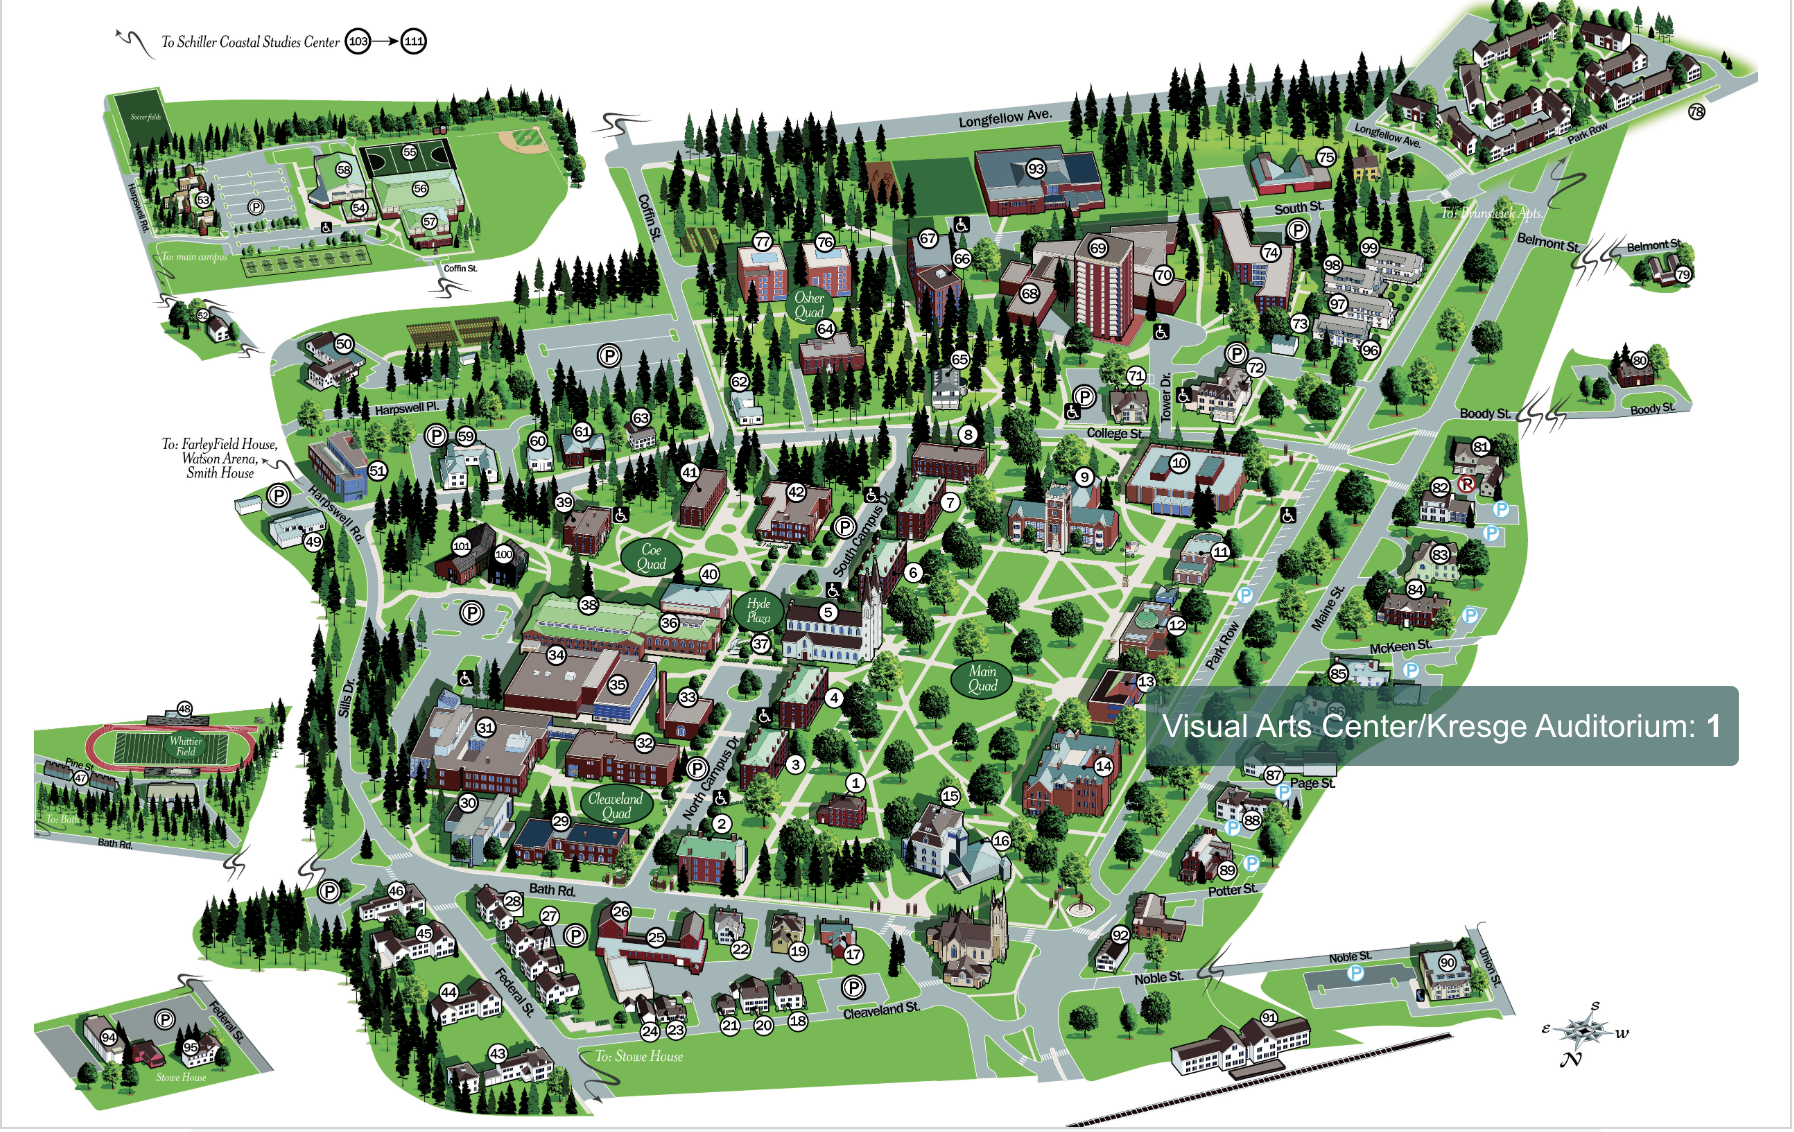
\includegraphics[width=0.5\linewidth]{HCI_Map.png}
    \includegraphics[width=0.5\linewidth]{HCI_Feed.png}
    \caption{Screenshots of the map and post list components of our app.}
    \label{fig:mapnfeed}
\end{figure}

\subsection{User Input and Engagement}

Users aren’t just looking at posts—they can make their own posts, and they can upvote or downvote other posts depending on whether they agree or disagree. These are the main affordances of our application, and they essentially act as the engine that makes it go. We think that this kind of interaction makes the app more satisfying to use, since people like being able to give their input.
We also added the ability for users to undo their vote if they change their mind or vote by accident (catering to Nielsen’s “User control and freedom” heuristic). However, users are still only limited to one total vote per post. This helps prevent people from spamming votes and keeps things more accurate, which is important since the goal is for admins to see real public opinion and act on it.

\subsection{Accurate Community Representation}

As mentioned above, we wanted the vote system to give an accurate depiction of the public opinion on campus. The one-vote limit helps with that. Also, the map shows how many posts each building has, which makes it clear where the most reports are coming from. That helps users focus on the more active areas, but more importantly, it helps campus leadership see which parts of campus need attention. The more posts a building has, the more likely it is that something there needs fixing.

\subsubsection{Navigation Bar}

\begin{figure}[htbp]
    \centering
    \includegraphics[width=0.5\linewidth]{HCI_Navigation_Bar.png}
    \caption{The Navigation Bar}
    \label{fig:navbar}
\end{figure}

The navigation bar includes: 

\begin{itemize}
    \item \textbf{Home} - which takes users to the map and feed view (this is the main page)
    \item \textbf{Make Post} – this brings up a pop-up form where users can write a post and choose a building. \autoref{fig:makepost}
    \item \textbf{Help} – this opens a help page that explains how to use the app. \autoref{fig:help}
\end{itemize}

\begin{figure}[htbp]

\centering
\begin{minipage}[h]{0.49\linewidth}    
    \centering
    \includegraphics[width=\linewidth]{HCI_Make_Post.png}
    \caption{The make post interface}
    \label{fig:makepost}
\end{minipage}
\hfill
\begin{minipage}[h]{0.49\linewidth}
    \centering
    \includegraphics[width=\linewidth]{HCI_Help_Page.png}
    \caption{Help page interface}
    \label{fig:help}
\end{minipage}
\end{figure}


The help page was a late addition to our app, but we believe that it is especially important because the app is only useful if the users know how to use it. We realized that we could not make any assumptions about our users’ knowledge of our platform and its different function. Nielsen also stresses this in one of his design heuristics (“Help and documentation”). The help page also consists of an email address for users to contact with any confusions they may have that aren’t addressed in the help documentation.

\newpage

\section{Methods}

\subsection{Participants}

For this study, we recruited 8 participants. Participants were selected by convenience sampling and consisted entirely of roommates of the authors. In order to minimize potential exposure to the design, the experiment was conducted in a separate room. This ensured that participants were not able to overhear other participants’ trials. Participants were also asked not to discuss their results with anyone who had not yet participated in the experiment. This prevented a culture of “speedrunning” from developing.

\subsection{Materials}

The experiment was conducted on one 13-inch, M2, MacBook Pro running macOS Sequoia 15.4. The experiment took place in Firefox Browser version 137.0.2. Both the frontend and the backend of the software were running locally, so latency was entirely eliminated. The Desktop version of the site was the website running on a full screen firefox tab. The Mobile version was run by using the Responsive Design Mode at 390x884 pixels. 

An additional note about this mac is that the owner uses it with the “Natural Scrolling” setting disabled. Every single participant in the experiment remarked on the fact that the scrolling was “backwards,” so as to eliminate this potential source of confusion, “Natural Scrolling” ought to be enabled in future tests.

To test the aesthetic qualities of the design, we utilized the Microsoft Desirability Toolkit vocabulary.\cite{noauthor_microsoft_nodate} Of the 118 words, we selected the following 8 words: \textbf{Fresh, Patronizing, Stressful, Clear, Rigid, Difficult, Accessible, Irrelevant, Advanced, Straight-forward}. Users were asked to select three of these words by using an ad hoc survey made with Google Sheets.

Finally, users were read a script during the experiment included in \autoref{a:tasks}. 

\subsection{Experiment Design}

The independent variable in this experiment was the website design version (Desktop vs Mobile). The dependent variables were the three descriptive words participants selected to reflect each design, as well as the time it took each user to complete each task. Each participant was tested on both designs, so the total number of participants is equal to the number who took part in each condition. 

We used a repeated-measures design because each participant interacted with both Desktop and Mobile versions of the design. We controlled for order effects via counterbalancing which design was shown first. This was done by simply alternating which design was shown first to each participant (desktop, mobile, desktop, mobile, etc.). Furthermore, primacy and recency effects were minimized in the design qualities list by randomizing the order in which the words appear each time a participant was exposed to the list. 

\subsection{Procedure}

Each user was first contacted to participate in the design. Then, at their convenience, I met with them in a private space of their choosing (Some were alone in the living room, kitchen, their room, etc.). The experimenter read each user the script included in Appendix (\autoref{a:tasks}). Users were timed from the time they were given the laptop to when they indicated they were done with the task. No matter what the user’s first design was, the interface was seeded with an existing complaint which read “Pothole outside of coleman” at the location Coleman Hall with 0 upvotes or downvotes. Screenshots of this are included in Appendix \autoref{a:init-state}. 

Between mobile and desktop (or vice versa), the post list was not reset, so the complaint/comment the user made on their first design would be present in the post list of the second design. After each data collection step, the computer was returned to the experimenter to record the data collected (timing information, selected words) on a separate spreadsheet and the design and questionnaire was reset accordingly

\newpage

\section{Results}

\subsection{Timing}

\begin{table}[ht]
\centering
\caption{User Design Interaction Times}
\begin{tabular}{llcc}
\toprule
Name & First design & Desktop time & Mobile time \\
\midrule
Jonathan & Desktop & 1:37.35 & 0:27.28 \\
Muhammed & Mobile & 0:29.78 & 0:47.92 \\
Christine & Desktop & 0:48.7 & 0:33.14 \\
Jordan & Mobile & 0:35.62 & 0:58.13 \\
Taylor & Desktop & 1:05.10 & 0:42.33 \\
Deva & Mobile & 0:41.80 & 0:50.07 \\
Avery & Desktop & 1:12.25 & 0:39.45 \\
Riley & Mobile & 0:38.93 & 0:44.66 \\
\bottomrule
\end{tabular}
\end{table}

The mean time it took for participants to complete the task on the \textbf{mobile} interface was 42.87 seconds. The mean time it took for participants to complete the task on the \textbf{desktop} version was 53.62 seconds. No matter which design was shown to the user, the participants completed the task on their second design faster. The mean time for users to complete the task on their first design was 60.39 seconds, and the mean time for the second design was 36.04 seconds.

A component that added time in the use of the design for many participants was them thinking about what complaint to type. For example, the participant nicknamed “Jonathan” spent a long time deliberating on what to type, whereas participant “Avery” simply typed “Mama Mia” into their complaint box. 

\subsection{Aesthetic}

\begin{table}[h!]
\centering
\caption{User Feedback on Designs}
\begin{tabular}{ll>{\raggedright\arraybackslash}p{4.5cm}>{\raggedright\arraybackslash}p{4.5cm}}
\toprule
Name & First design & Desktop words & Mobile words \\
\midrule
Jonathan & Desktop & Accessible, Clear, Straightforward & Accessible, Clear, Straightforward \\
Muhammed & Mobile & Accessible, Straightforward, Clear & Rigid, Difficult, Straight forward \\
Christine & Desktop & Accessible, Straightforward, Clear & Difficult, Straightforward, Clear \\
Jordan & Mobile & Clear, Accessible, Fresh & Difficult, Rigid, Stressful \\
Taylor & Desktop & Straight forward, Clear, Rigid & Straight forward, Accessible, Fresh \\
Deva & Mobile & Patronizing, Advanced, Stressful & Straight forward, Clear, Accessible \\
Avery & Desktop & Accessible, Clear, Advanced & Irrelevant, Stressful, Rigid \\
Riley & Mobile & Clear, Difficult, Rigid & Straight forward, Accessible, Clear \\
\bottomrule
\end{tabular}
\end{table}

The top five words overall were Clear (11), Straightforward (10), Accessible (9), Rigid (5), and Difficult (4). The top five words for the Desktop site were Clear (7), Accessible (5), Straightforward (4), Rigid (2), and Advanced (2). For the mobile site, the top five words were Straightforward (6), Accessible (4), Clear (4), Rigid (3), and Difficult (3). The most significant difference between desktop and mobile was that users felt the desktop interface was “Advanced” while they found the mobile interface “Difficult”. 

\begin{figure}[h!]
    \centering
    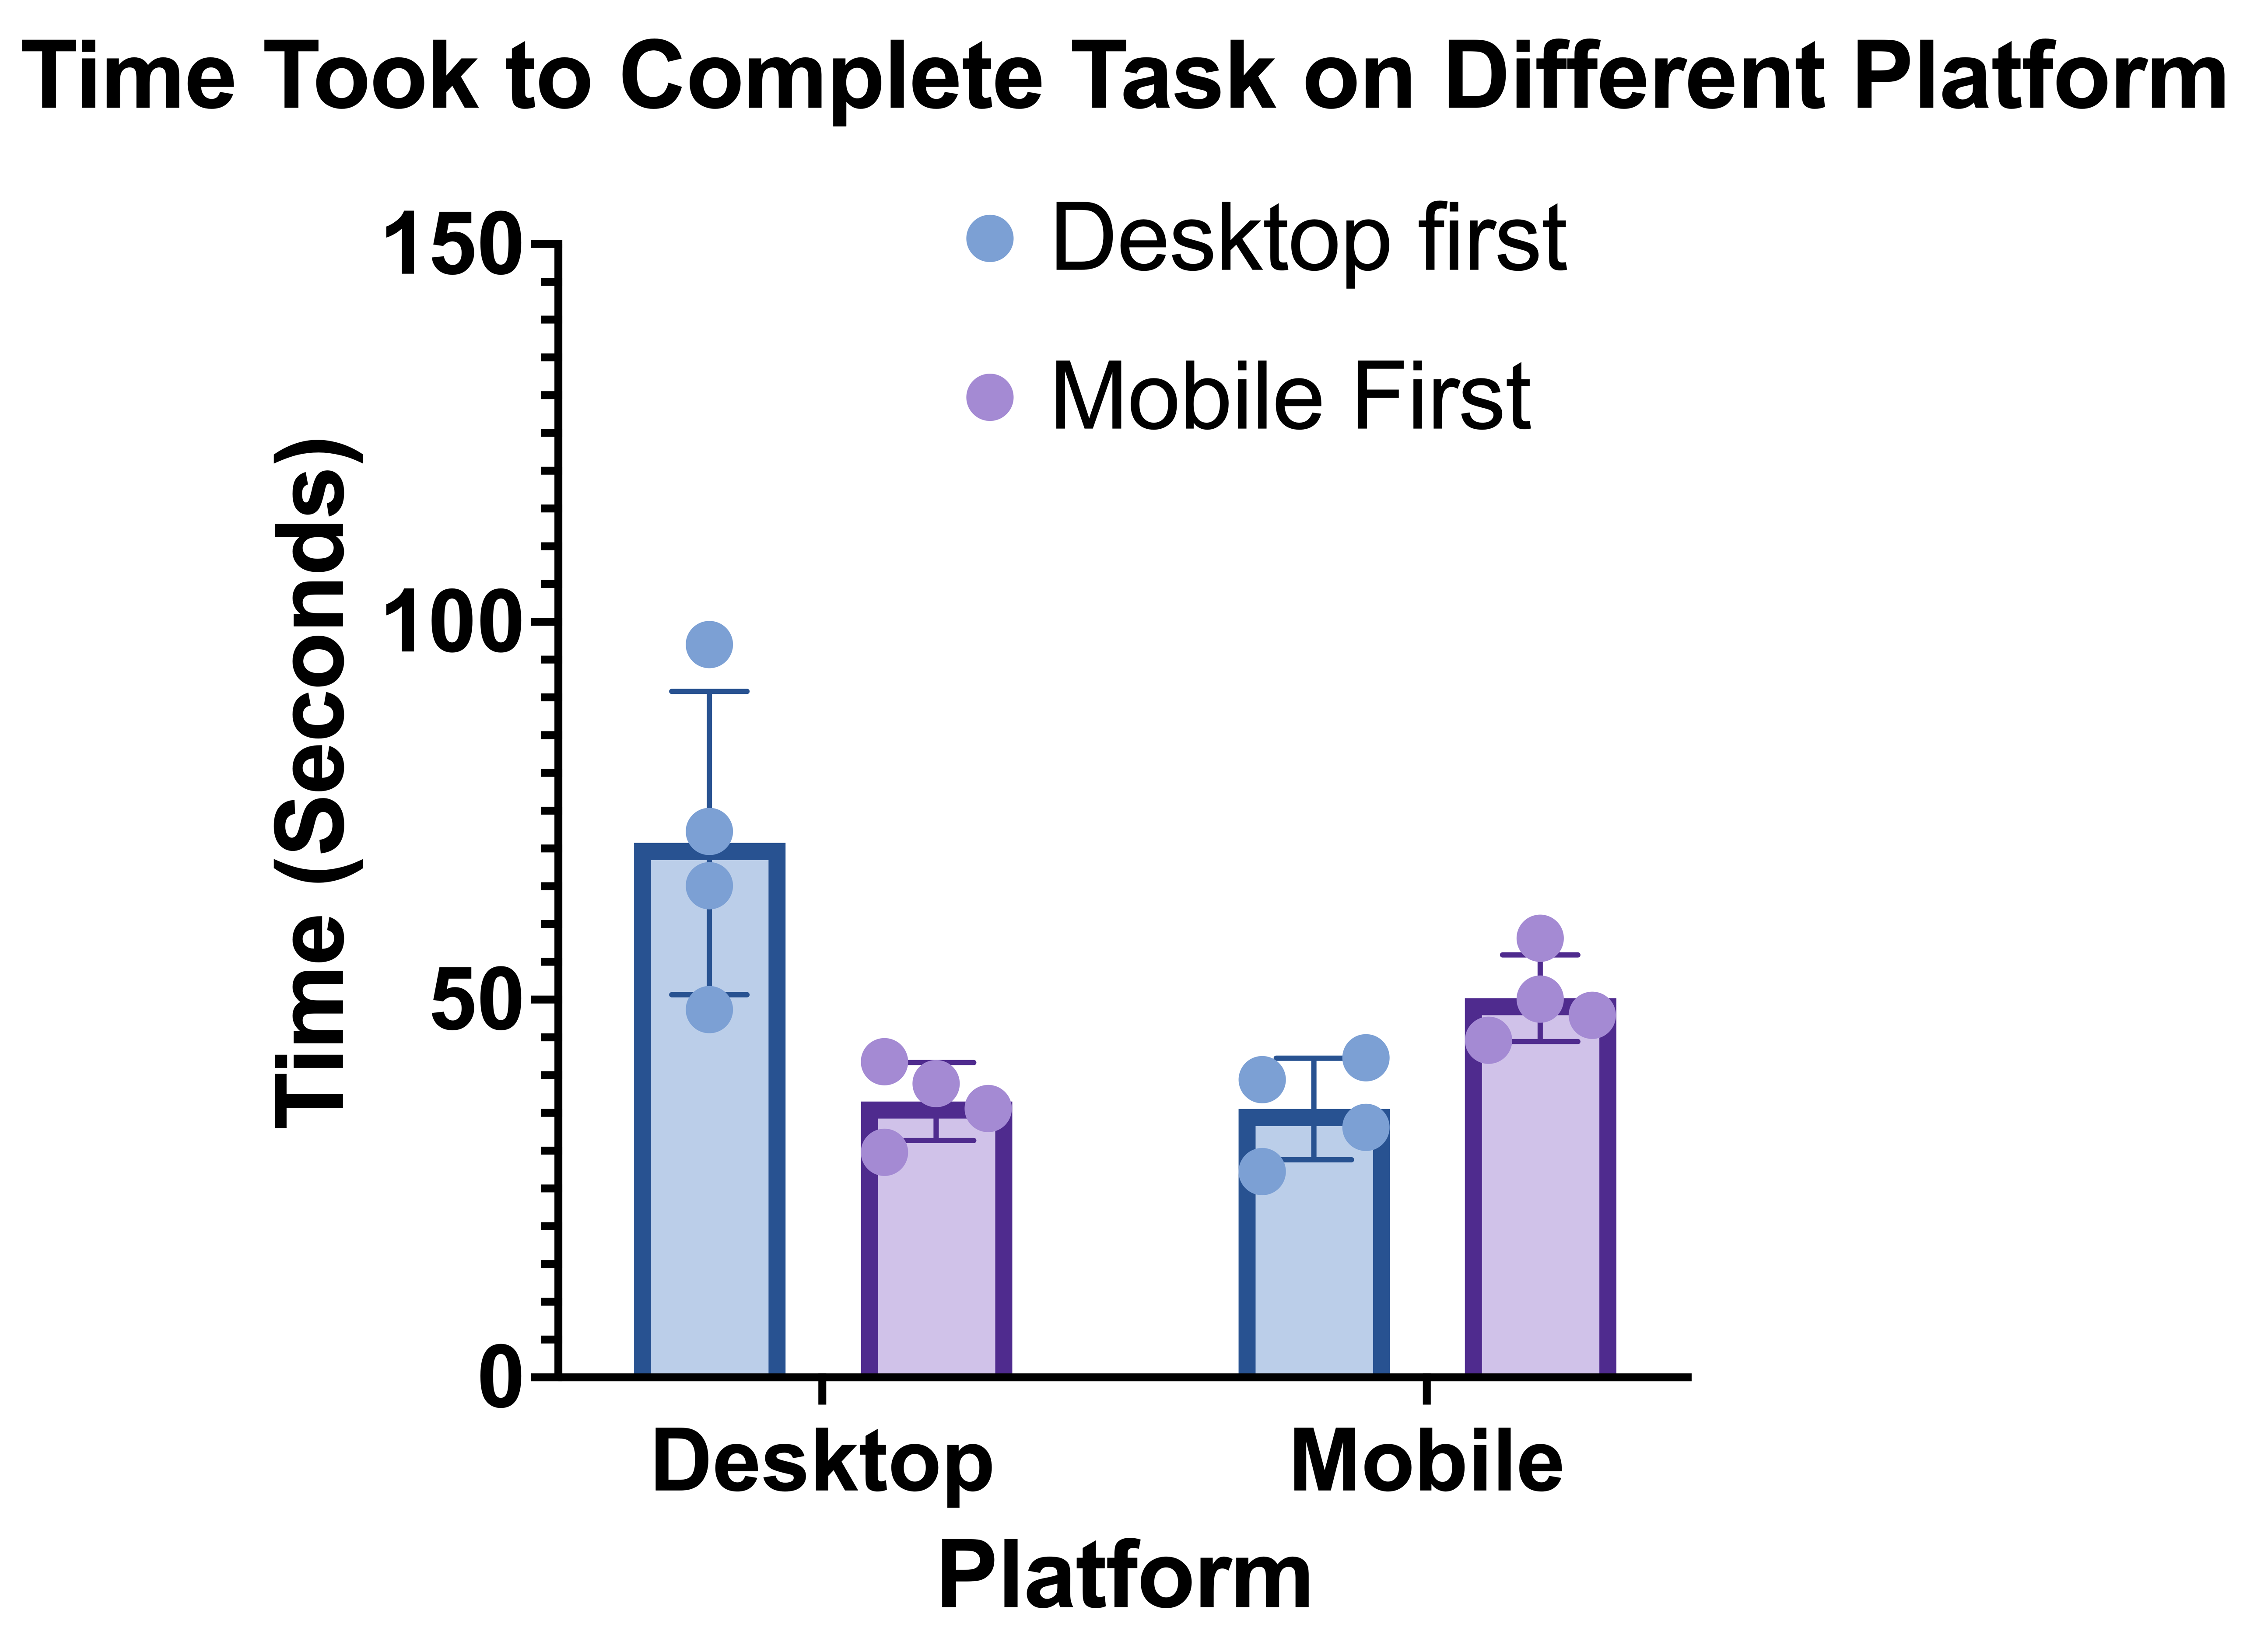
\includegraphics[width=0.5\linewidth]{results.png}
    \caption{Comparison of average time took to complete the task. }
    \label{fig:1}
\end{figure}

\newpage

\section{Discussion}

\subsection{Looking Back}

The results of this study revealed several meaningful patterns among both the desktop and mobile design for our application. Overall participants tended to complete the task on the mobile device slightly more quickly. However, regardless of which design the participant started with they completed the task on the second design significantly quicker. This suggests the presence of a practice or familiarity effect that transfers across designs. This insight also tempers the claim that the mobile design was universally faster, as learning from the first experience carried over and allowed those who completed the mobile task first to subsequently complete the desktop design faster. 


Aesthetically, users described both designs as being “Clear”, “Straightforward”, and “Accessible”, suggesting that participants found the design relatively easy to understand and navigate. However, the mobile design was also described as “Difficult”, an adjective that was not mentioned in regards to the mobile design. This difference is likely due to the hamburger menu that hides the “Make Post” button on the mobile design. Users likely found it difficult to determine where to navigate on the site in order to make a post, particularly in comparison to the desktop design. This indicates that despite the mobile design being more efficient for task completion there are still some usability challenges that need to be addressed.


These results align with our initial expectation that the mobile design might support faster interactions and task completion, but also reveal important nuances in human perception that goes beyond speed. Our findings extend previous research in human-computer interactions suggesting efficiency is not always aligned with perceived usability. While the faster completion times seem to suggest higher usability, there were still aspects to the design that users found more rigid and difficult compared to the desktop design.


Several methodological limitations must be acknowledged and addressed. The small and homogenous participant pool limits the generalizability of this study. The use of Firefox’s responsive design mode to emulate mobile usage may not accurately reflect real world mobile applications, as users were still typing and using the touchpad rather than using a touchscreen interface. A major factor in the time it took users to complete the task was the amount of time they spent thinking of the content for their post. This is something that we should have controlled for as it was not a reflection of the design itself but may have still had a major impact on the results.

\subsection{Looking Forward}

These findings have implications for the design of cross-platform web applications. They highlight the tension between optimizing speed and optimizing for perceived usability and control. While mobile layouts may tend to encourage faster execution they do run the risk of being perceived as more difficult to use and more constrained. Designers must be cautious to not direct all focus towards efficiency and instead receive user feedback throughout the design process, allowing them to focus on creating a user-friendly experience. 


For future research, expanding the participant pool to include people from a wider range of backgrounds, particularly with different levels of technological proficiency, will provide more robust and generalizable results. Additionally, conducting the mobile part of the experiment on an actual mobile device rather than a laptop would make the results more difficult to undermine. Lastly, the time participants spent thinking of what to type could be controlled for by providing predefined text for them to type. This would eliminate that uncontrolled variable and provide more consistent data. It could also be worth running the experiment with slight visual modifications to see how that changes user perception.

\newpage

\section{Conclusion}

In summary, the study found that users tended to complete the task more quickly on the mobile design, but perceived the desktop design as being less difficult to work with. These findings suggest that mobile design can increase efficiency, but they must be designed carefully with regards to user perception, as this can vary from efficiency. Despite some methodological constraints the study does offer valuable insight into the tradeoff between efficiency and usability. It also demonstrates how the familiarity effect can transfer across different platforms and layouts when the functionality remains the same. Future research should continue to refine measurement techniques and design strategy to balance the different aspects of the user experience.


\bibliographystyle{plain}
\bibliography{hci}

\newpage 

\appendix

\section{Appendix}

\subsection{Script for Tasks}
\label{a:tasks}

Hi, thanks for helping us out today! We’re testing an early version of our website, where users can make and interact with posts about campus-wide issues. It should only take a few minutes or less to complete. I’ll ask you to create a new post by clicking “Make Post” and filling out the information from there. Do you have any questions about completing this task? 

** let them complete the task ** 

Now I will show you a list of words. Please select three words that you believe reflects this design

**Let them select three words**

Next, I will ask you to perform the same task on a different design.

** let them complete the task ** 

Once again I will show you a list of words. Please select three words that you believe reflects this design

Thank you so much for your time! If you have any questions, please feel free to reach out to us.

\subsection{Initial state of Mobile and Desktop Design
}
\label{a:init-state}

\begin{figure}
    \centering
    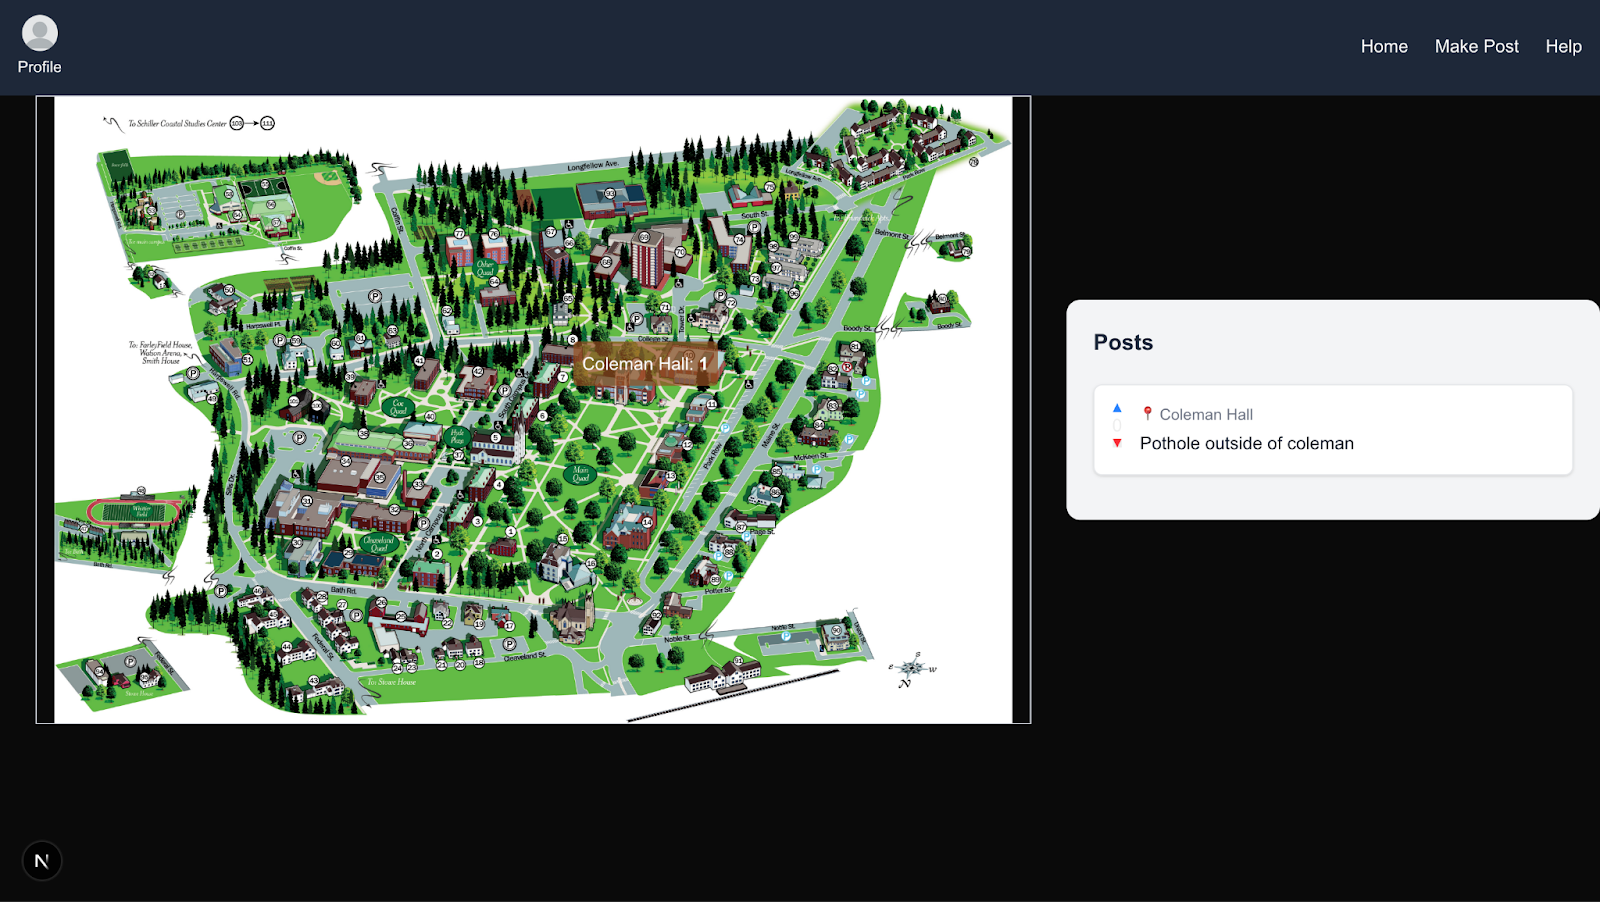
\includegraphics[width=0.5\linewidth]{desktop.png}
    \caption{Initial Desktop Interface}
    \label{fig:desktop}
\end{figure}

\begin{figure}
    \centering
    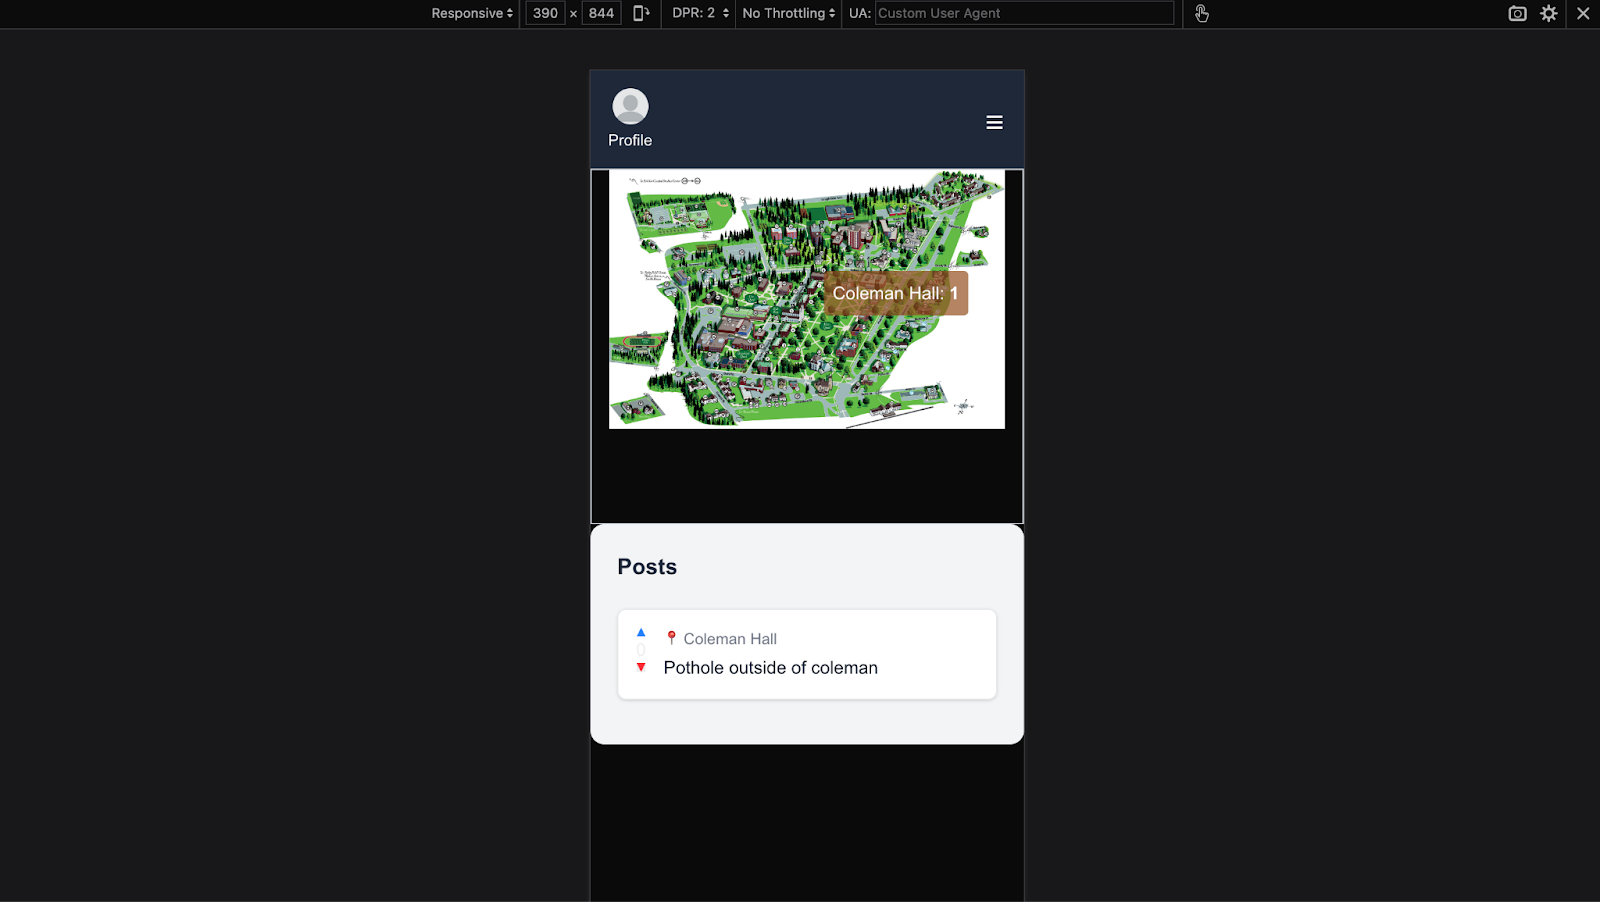
\includegraphics[width=0.5\linewidth]{mobile.png}
    \caption{Initial Mobile Interface}
    \label{fig:mobile}
\end{figure}

\newpage

\section{Acknowledgments}
Professor Harmon! 

\end{document}
